% Drawing 154/02-1 -- folder 154, batch 02, archive page 21 (PDF page 22).
% Transcription: figure, en haut à gauche : un arc (en vert) longé de part et d'autre par deux arcs bruns, traversé par six faisceaux de pseudo-droites orange ; sur les arcs bruns, des segments épais noirs marquent les arcs découpés à chaque croisement
% Kind: arc with parallel arcs crossed by pencils. Method 2 (schematic redraw from the facsimile). Status: ok.
% Notes: A green arc flanked on both sides by brown arcs, crossed by pencils of orange pseudolines; thick black strokes on the brown arcs mark the arcs cut off at each crossing. Seven crossings are visible on the facsimile (the two at the right end close together); the transcription counts six fans. The figure stands at the top of the right half of the sheet.
% Coordinates: 1 unit = 1 mm = 1/100 of the crop width (bbox in page fractions: [0.506, 0.079, 0.764, 0.191]).
% Redrawn by Claude (claude-opus-5-5), issue #73, 2026-11-07; not checked by a human; not compiled (no TeX in the session).
% Revised by Claude (claude-opus-5-5) 2026-11-09 (issue #128) after Michel's check: vertices snapped to exact intersections (drawn points on their lines, meeting ends on the stroke they meet, near-concurrent lines through one computed point, curve ends on their rim); labels at \small as in folder 80 batch 3. Status: ok.
% Rights: reproduces part of the work -- behind RENDER_TRANSCRIPTS, never published by itself.
\documentclass[tikz,border=3pt]{standalone}
\usepackage{amsmath,amssymb}
\usetikzlibrary{patterns,arrows.meta}
\tikzset{Or/.style={orange!90!black}, Ye/.style={yellow!80!orange}, Lg/.style={green!60!black!70}, Dg/.style={green!45!black}, Br/.style={brown!80!black}, Rd/.style={red!85!black}, Bl/.style={blue!70!black}, Gy/.style={black!40}, pencil/.style={black!45}, struck/.style={black!35}, mark/.style={circle,draw,inner sep=1.3pt}, pt/.style={circle,fill,inner sep=0.9pt}, opt/.style={circle,draw,fill=white,inner sep=1.1pt}}
\colorlet{Or}{orange!90!black}\colorlet{Ye}{yellow!80!orange}\colorlet{Lg}{green!60!black!70}\colorlet{Dg}{green!45!black}\colorlet{Br}{brown!80!black}\colorlet{Rd}{red!85!black}\colorlet{Bl}{blue!70!black}\colorlet{Gy}{black!40}
\begin{document}
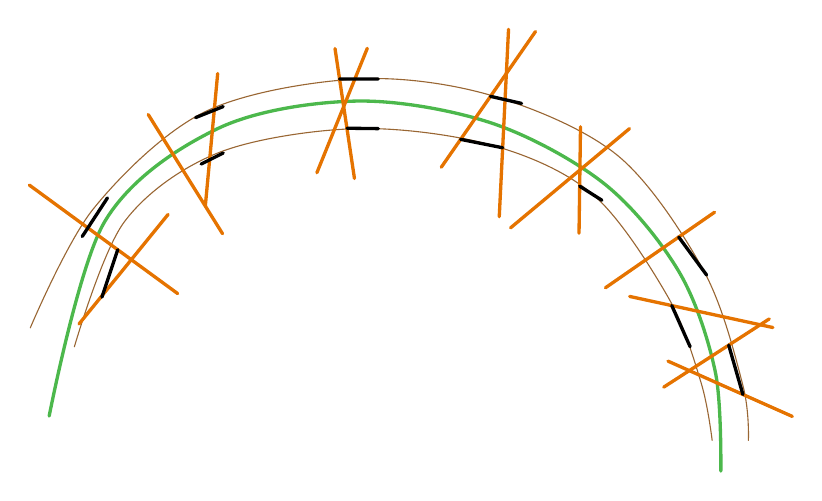
\begin{tikzpicture}[x=1mm,y=1mm,line cap=round,line join=round,font=\scriptsize]
\draw[Lg,very thick] plot[smooth, tension=0.55] coordinates {(4.2,-51.6) (11.2,-27) (25.6,-15.1) (43.2,-11.6) (60.4,-14.4) (74.7,-22.1) (84.2,-33.3) (88.8,-46) (89.5,-58.6)};
\draw[Br] plot[smooth, tension=0.55] coordinates {(1.8,-40.4) (9.8,-25.3) (23.9,-13) (43.2,-8.8) (60.4,-10.9) (76.5,-18.6) (87.4,-33.3) (92.3,-47.7) (93,-54.7)};
\draw[Br] plot[smooth, tension=0.55] coordinates {(7.4,-42.8) (13.7,-27) (25.6,-18.2) (43.2,-15.1) (60.4,-17.2) (73.3,-23.5) (82.8,-36.5) (87,-47.4) (88.4,-54.7)};
\draw[Or,very thick] (1.68,-22.27) -- (20.52,-36.05);
\draw[Or,very thick] (19.3,-26) -- (7.99,-39.91);
\draw[Or,very thick] (16.78,-13.31) -- (26.22,-28.45);
\draw[Or,very thick] (25.6,-8.1) -- (24.03,-24.93);
\draw[Or,very thick] (40.5,-4.93) -- (42.97,-21.43);
\draw[Or,very thick] (44.6,-4.9) -- (38.2,-20.7);
\draw[Or,very thick] (65.96,-2.77) -- (54,-20);
\draw[Or,very thick] (62.54,-2.49) -- (61.36,-26.28);
\draw[Or,very thick] (77.9,-15.1) -- (62.8,-27.7);
\draw[Or,very thick] (71.68,-14.86) -- (71.49,-28.39);
\draw[Or,very thick] (88.7,-25.72) -- (74.85,-35.31);
\draw[Or,very thick] (77.92,-36.41) -- (96.11,-40.36);
\draw[Or,very thick] (95.65,-39.27) -- (82.25,-47.93);
\draw[Or,very thick] (82.79,-44.63) -- (98.58,-51.65);
\draw[very thick] (8.4,-28.8) -- (11.6,-23.9);
\draw[very thick] (22.8,-13.7) -- (26.3,-12.3);
\draw[very thick] (41.08,-8.79) -- (46,-8.8);
\draw[very thick] (60.24,-11) -- (64.2,-11.9);
\draw[very thick] (84.15,-28.87) -- (87.7,-33.7);
\draw[very thick] (90.5,-42.6) -- (92.3,-48.86);
\draw[very thick] (12.9,-30.48) -- (10.9,-36.5);
\draw[very thick] (23.5,-19.6) -- (26.3,-18.2);
\draw[very thick] (42.02,-15.05) -- (46,-15.1);
\draw[very thick] (56.45,-16.46) -- (61.8,-17.53);
\draw[very thick] (71.57,-22.41) -- (74.4,-24.2);
\draw[very thick] (83.27,-37.57) -- (85.6,-42.8);
\end{tikzpicture}
\end{document}
